\documentclass[tikz,border=2pt]{standalone}
\usepackage{amsmath}
\usepackage{pgfplots}
\pgfplotsset{compat=1.18}
\usetikzlibrary{arrows.meta}
\begin{document}
% Exercise 6.10 step (b): tableau after x1 replaced x5 in Example 6.3; negative reduced costs at x2 (-1) and x4 (-0.75),
% smallest index 2 -> x2 enters; ratios 0/0.5 = 0 and 0/2.5 = 0 tie between x1 and x6; Bland: smallest index 1 -> x1 leaves
% (then x3 has column (-7,-2): unbounded), whereas the lower-row rule lets x6 leave and continues the cycle.
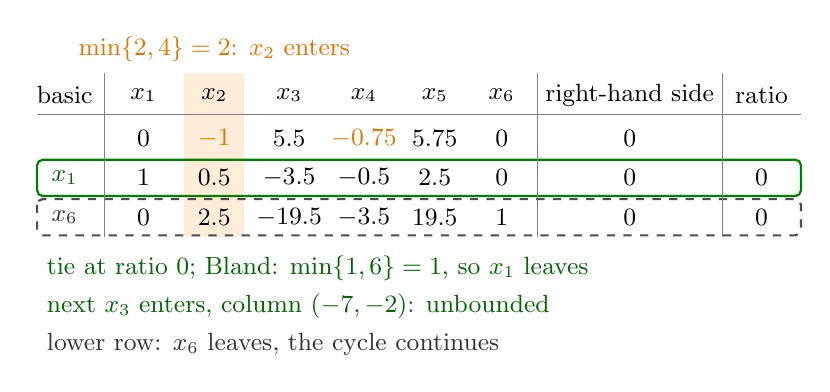
\begin{tikzpicture}[font=\small, >={Latex[length=2mm]}]
  % highlights
  \fill[orange!15] (1.52,0.28) rectangle (2.28,-1.8);
  \draw[green!50!black, thick, rounded corners=2pt] (-0.35,-0.82) rectangle (9.35,-1.28);
  \draw[gray!60!black, thick, dashed, rounded corners=2pt] (-0.35,-1.32) rectangle (9.35,-1.78);
  % header
  \node at (0,0) {basic};
  \foreach \j/\x in {1/1.0,2/1.9,3/2.85,4/3.8,5/4.7,6/5.55} \node at (\x,0) {$x_{\j}$};
  \node at (7.175,0) {right-hand side};
  \node at (8.85,0) {ratio};
  \draw[gray] (-0.35,-0.25) -- (9.35,-0.25);
  \draw[gray] (0.5,0.28) -- (0.5,-1.8) (6.0,0.28) -- (6.0,-1.8) (8.35,0.28) -- (8.35,-1.8);
  % objective row
  \node at (1.0,-0.55) {$0$};
  \node[orange!90!black] at (1.9,-0.55) {$-1$};
  \node at (2.85,-0.55) {$5.5$};
  \node[orange!90!black] at (3.8,-0.55) {$-0.75$};
  \node at (4.7,-0.55) {$5.75$};
  \node at (5.55,-0.55) {$0$};
  \node at (7.175,-0.55) {$0$};
  % row x1
  \node[green!40!black] at (0,-1.05) {$x_1$};
  \foreach \v/\x in {1/1.0,0.5/1.9,-3.5/2.85,-0.5/3.8,2.5/4.7,0/5.55} \node at (\x,-1.05) {$\v$};
  \node at (7.175,-1.05) {$0$};
  \node at (8.85,-1.05) {$0$};
  % row x6
  \node[gray!40!black] at (0,-1.55) {$x_6$};
  \foreach \v/\x in {0/1.0,2.5/1.9,-19.5/2.85,-3.5/3.8,19.5/4.7,1/5.55} \node at (\x,-1.55) {$\v$};
  \node at (7.175,-1.55) {$0$};
  \node at (8.85,-1.55) {$0$};
  % entering: smallest index
  \node[orange!90!black, anchor=south] at (1.9,0.3) {$\min\{2,4\}=2$: $x_2$ enters};
  % leaving: tie, smallest index
  \node[anchor=west, green!40!black] at (-0.35,-2.2) {tie at ratio $0$; Bland: $\min\{1,6\}=1$, so $x_1$ leaves};
  \node[anchor=west, green!40!black] at (-0.35,-2.68) {next $x_3$ enters, column $(-7,-2)$: unbounded};
  \node[anchor=west, gray!40!black] at (-0.35,-3.16) {lower row: $x_6$ leaves, the cycle continues};
\end{tikzpicture}
\end{document}
